\chapter{Norms}
The essential notions of size and distance in a vector space are captured by norms. These are the yardsticks with which we measure approximations and convergence throughout numerical linear algebra.

\section{Vector Norms}

%────────────────────────────────────────
\begin{definition}
[Norm]
\label{def: Norm}
A norm is a function $\|\cdot\|: \mathbb{C}^m \rightarrow \mathbb{R}$ that assigns a real-valued length to each vector. In order to conform to a reasonable notion of length, a norm must satisfy the following three conditions. For all vectors $x$ and $y$ and for all scalars $\alpha \in \mathbb{C}$,
\begin{itemize}
    \item $\|x\| \geq 0$, and $\|x\|=0$ only if $x=0$,
    \item $\|x+y\| \leq\|x\|+\|y\|$,
    \item $\|\alpha x\|=|\alpha|\|x\|$.
\end{itemize}
\end{definition}
%────────────────────────────────────────

The most important class of vector norms, the $p$-norms, are defined below. The closed unit ball $\left\{x \in \mathbb{C}^m:\|x\| \leq 1\right\}$ corresponding to each norm is illustrated to the right for the case $m=2$.

%────────────────────────────────────────
\begin{figure}[H]
    \centering
    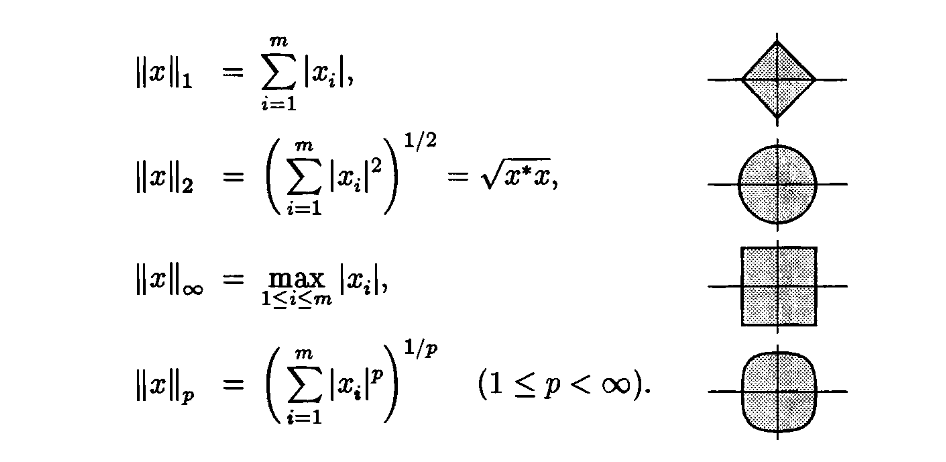
\includegraphics[width=0.7\textwidth]{figures/3-1.png}
\end{figure}
%────────────────────────────────────────

\section{Induced Matrix Norms} 
An $m \times n$ matrix can be viewed as a vector in an $m n$-dimensional space: each of the $m n$ entries of the matrix is an independent coordinate. Any $m n$ dimensional norm can therefore be used for measuring the ``size'' of such a matrix. However, in dealing with a space of matrices, certain special norms are more useful than the vector norms already discussed. These are the induced matrix norms, defined in terms of the behavior of a matrix as an operator between its normed domain and range spaces. 

Given vector norms $\|\cdot\|_{(n)}$ and $\|\cdot\|_{(m)}$ on the domain and the range of $A \in \mathbb{C}^{m \times n}$, respectively, the induced matrix norm $\|A\|_{(m, n)}$ is
\[
    \|A\|_{(m, n)}=\sup _{\substack{x \in \mathbb{C}^n \\ x \neq 0}} \frac{\|A x\|_{(m)}}{\|x\|_{(n)}}=\sup _{\substack{x \in \mathbb{C}^n \\\|x\|_{(n)}=1}}\|A x\|_{(m)}. 
\]

\section{Cauchy-Schwarz and H\"older Inequalities} 
Computing matrix $p$-norms with $p \neq 1, \infty$ is more difficult, and to approach this problem, we note that inner products can be bounded using $p$-norms. Let $p$ and $q$ satisfy $1 / p+1 / q=1$, with $1 \leq p, q \leq \infty$. Then the Hölder inequality states that, for any vectors $x$ and $y$,
\begin{align}
    \label{eq: Holder}
\left|x^* y\right| \leq\|x\|_p\|y\|_q
\end{align}
The Cauchy-Schwarz inequality is the special case $p=q=2$ :
\begin{align}
    \label{eq: cauchy}
\left|x^* y\right| \leq\|x\|_2\|y\|_2
\end{align}
Derivations of these results can be found in linear algebra texts. Both bounds are tight in the sense that for certain choices of $x$ and $y$, the inequalities become equalities.

\section{Bounding $\|AB\|$ in an Induced Matrix Norm} 
Computing matrix $p$-norms with $p \neq 1, \infty$ is more difficult, and to approach this problem, we note that inner products can be bounded using $p$-norms. Let $p$ and $q$ satisfy $1 / p+1 / q=1$, with $1 \leq p, q \leq \infty$. Then the Hölder inequality states that, for any vectors $x$ and $y$,
\begin{align*}
\left|x^* y\right| \leq\|x\|_p\|y\|_q
\end{align*}
The Cauchy-Schwarz inequality is the special case $p=q=2$ :
\begin{align*}
\left|x^* y\right| \leq\|x\|_2\|y\|_2
\end{align*}
Derivations of these results can be found in linear algebra texts. Both bounds are tight in the sense that for certain choices of $x$ and $y$, the inequalities become equalities.

\section{General Matrix Norms}
As noted above, matrix norms do not have to be induced by vector norms. In general, a matrix norm must merely satisfy the three vector norm conditions applied in the $m n$-dimensional vector space of matrices:
\begin{itemize}
    \item $\|A\| \geq 0$, and $\|A\|=0$ only if $A=0$,
    \item $\|A+B\| \leq\|A\|+\|B\|$,
    \item $\|\alpha A\|=|\alpha|\|A\|$.
\end{itemize}
The most important matrix norm which is not induced by a vector norm is the \textbf{Hilbert-Schmidt} or \textbf{Frobenius norm}, defined by
\begin{align*}
\|A\|_F=\left(\sum_{i=1}^m \sum_{j=1}^n\left|a_{i j}\right|^2\right)^{1 / 2} .
\end{align*}
Observe that this is the same as the 2-norm of the matrix when viewed as an $m n$-dimensional vector. The formula for the Frobenius norm can also be written in terms of individual rows or columns. For example, if $a_j$ is the $j$ th column of $A$, we have
\begin{align*}
\|A\|_F=\left(\sum_{j=1}^n\left\|a_j\right\|_2^2\right)^{1 / 2}
\end{align*}
This identity, as well as the analogous result based on rows instead of columns, can be expressed compactly by the equation
\begin{align*}
\|A\|_F=\sqrt{\operatorname{tr}\left(A^* A\right)}=\sqrt{\operatorname{tr}\left(A A^*\right)}. 
\end{align*}
Note that 
\[
    \|AB\|_F^2 \le \|A\|_F^2 \|B\|_F^2. 
\]

\section{Invariance under Unitary Multiplication} 

%────────────────────────────────────────
\begin{theorem}
\label{thm: invar under unitary multiplication}
 For any $A \in \mathbb{C}^{m \times n}$ and unitary $Q \in \mathbb{C}^{m \times m}$, we have
\begin{align*}
\|Q A\|_2=\|A\|_2, \quad\|Q A\|_F=\|A\|_F. 
\end{align*}
\end{theorem}
%────────────────────────────────────────
